\chapter{Introduction} \label{sec:introduction}
\epigraphhead[50]{\epigraph{%
\textit{"A planet is the cradle of mind, but one cannot live in a cradle forever."}}%
{\textsc{Konstantin E. Tsiolkovsky (1857 - 1935)}}%
}

\section{The conquest of space} \label{sec:conquest}

Since in 1609 German mathematician and astronomer Johannes Kepler published his book \textit{Astronomia nova}, containing the most famous of all transcendental equations, the motion of the celestial bodies has attracted the attention of the greatest minds in human history, even sparkling entire new fields in mathematics \cite{battin1999introduction}. It is easy to imagine that if even Kepler's equation, the one that captures the essence of the two-body problem in its most restricted form, already has this mathematical intricacy, any further development will carry away similar or greater complexity.

\begin{figure}[h]
\[M = E - e \sin{E}\]
\caption{The Kepler equation.}
\end{figure}

Almost three centuries later, in 1903, Russian rocket scientist Konstantin E. Tsiolkovsky first explained in his article \textit{Exploration of Outer Space by Means of Rocket Devices} precise conditions for artificial objects to reach the orbit of the Earth, making a huge leap from the mere observation of the celestial bodies and the science fiction stories that had inspired him to the real possibility of going to space. Quoting \cite{siddiqi2000challenge}:

\begin{displayquote}
In his most revolutionary idea, he proposed that humans could hope to fly to very high altitudes and ultimately into outer space only by using liquid-propellant rockets. One of his most  important conclusions was that a rocket would be capable of carrying up a cargo of any size, and develop any speed desired,  as long as the rocket was sufficiently large and the ratio of the mass of the propellant to the mass of the entire rocket was  large enough -- a relationship that is known as the Tsiolkovsky Equation.
\end{displayquote}

% Regarding Saxon genitive and equation names
% http://english.stackexchange.com/a/301270/20057

\begin{figure}[h]
\[\Delta v = v_\text{e} \ln \frac {m_0} {m_f}\]
\caption{The Tsiolkovsky equation.}
\end{figure}

If we define the term Astrodynamics as the branch of Mechanics that studies practical problems concerning the motion of rockets and other artificial objects through space, Tsiolkovsky's contribution might well be considered its starting point, and many others ensued before they could be tested in practice during the second half of the 20th century. In 1919 Yuri V. Kondratyuk conceived the gravitational slingshot or flyby to accelerate a spacecraft through interplanetary flight and suggested a mission profile for a Lunar landing \cite{siddiqi2000challenge}, in 1925 Walter Hohmann conjectured that the minimum-fuel transfer between two coplanar circular orbits consists of two tangent impulses along the line of apses (although this result was not proved until almost forty years later in \cite{lawden1963optimal}) and in 1926 Hermann J. Oberth observed that the velocity gain of an impulsive maneuver is higher kinetic energy is maximum (nowadays known as the Oberth effect). The severe limitations in weight and available energy for such kind of travels were already apparent for these pioneers, who were, in some way, anticipating the need to optimize on board fuel consumption.

At the same time, important practical advances were being made in the field of rocketry. In 1920 Robert H. Goddard published in his article \textit{A Method of Reaching Extreme Altitudes} several ideas and experimental results regarding the study of rockets, in particular that the exhaust speed of their combustion gases could be greatly increased by using convergent-divergent or De Laval nozzles, and in 1926 he launched the world's first liquid-fueled rocket, which reached an altitude of 12 meters, lasted 2 seconds and averaged about 100 kilometers per hour. After this remarkable event, amateur rocket societies started to form in America and Europe and bigger and more sophisticated rockets were built and launched in the following years.

To this day, chemical propulsion (whether using liquid fuel as pioneered by Goddard and later used by the Saturn V or solid fuel as already used by the Chinese in the 13th century) continues to be the only way to escape the gravitational well of the Earth. What is not so well known is that many of the people involved in the early development of astrodynamics and astronautics in the 20th century shared a common interest in an alternative method: electric propulsion. Goddard had already reflected on the use of "electrons moving with the velocity of light" as a method of propulsion as early as 1906, and Tsiolkovski wrote in 1911 about the use of electricity "to produce a large velocity for the particles ejected from a rocket device" \cite{choueiri2004history}. Oberth even envisioned electric propulsion as a real possibility for attitude control in his 1929 book \textit{Ways to Spaceflight} and already predicted its mass saving capabilities.

Despite all this enthusiasm, however, there were far too many obstacles at the time to make it a reality: first of all, the understanding of atomic physics was still in its infancy, with the nature of the electrons still unclear and the discovery of the proton not happening until 1920, hindering rigorous studies. Besides, electric propulsion was definitely not useful to attain orbital velocity, and on the other hand it requires a much more complex mathematical analysis (we will expand on these aspects in \ref{sec:propulsion}). For the following fifteen years after the publication of Oberth's book all the focus shifted away from electrical propulsion, until the tremendous advances regarding the production of intense ion currents during the forties brought back the debate about its feasibility \cite{choueiri2004history}.

In 1950 George F. Forbes presented the element that was missing for a complete mathematical analysis, the study of low-thrust trajectories, by showing for the first time that in some cases they were more efficient than the high-thrust counterparts in his Masters thesis \textit{The trajectory of a powered rocket in space}. This, and the contribution of Lyman S. Spitzer, who in his 1952 paper \textit{Interplanetary Travel Between Satellite Orbits} suggested that for an ion propulsion system to be technically useful an acceleration of three centimeters per square second would be enough ("sufficient to attain a velocity of $15~\text{km/sec}$ in two months" \cite{spitzer1952interplanetary}), provided the building blocks for the electrical propulsion to have the attention it deserved.

Finally, the decade of the sixties served as the definitive \textit{tour de force} of chemical propulsion, which powered the rockets used during the space race that started in 1957 with the launch of Sputnik I by the Soviet Union and that culminated with in 1969 with the first manned landing on the Moon by the United States of America. In the meanwhile, in 1964 the first mission to demonstrate the use in orbit of an ion thruster, SERT-1, was launched, whereas a milestone comparable in importance arrived as late as 1998 with the mission Deep Space 1. With these achievements the early ideas of the visionaries of the beginning of the century were finally proven real, and humanity was in the position of using these technologies to "leave the cradle".

\section{Chemical versus electric propulsion} \label{sec:propulsion}

After the historical perspective given in \ref{sec:conquest} we dedicate the following sections to introduce some important theoretical concepts, with the objective of justifying the importance of low-thrust orbit analysis within the context of orbit optimization and the pursuit of analytical solutions in this area. We start with the distinction of chemical versus electric propulsion and the main similarities and differences between them -- this does not intend to be an in-depth description of the subsystems and technologies that are involved, but rather an overview of their most essential aspects and how do they affect their performance and use cases (for such in-depth analysis we direct the readers to well known references in the subject such as \cite{sutton2016rocket}). In \ref{sec:methodstable} a thorough list of spacecraft propulsion methods has been included for reference.

Except for very small satellites, nearly all space missions require on-board propulsion systems, which have a major impact on spacecraft mass \cite{curran1993nasa}. Some sources estimate that the current cost of sending one kilo of payload into low Earth orbit lies around 20~000~€, and therefore any effort to decrease the launch mass of the spacecraft leads to significant savings \cite{choueiri2009new}.

We can define propulsion in a broad sense as the act of changing the motion of a body \cite{sutton2016rocket}. Spacecraft propulsion methods can be classified according to the energy source that is used to produce thrust, which can be chemical, nuclear or electric.

\textbf{Chemical propulsion} uses the chemical potential stored in the propellants, usually of reducing (fuel) and oxidizing nature, that is released in a high-pressure combustion reaction between the two. The reaction produces a flow of hot gases (between 2500 and 4100~\celsius) that can be accelerated in a convergent-divergent (or De Laval) nozzle to achieve supersonic velocities (1800 to 4300 m/s). In this case, therefore, the power source and the propellants are the same elements. Chemical propulsion systems can be themselves subdivided according to the state of the propellants: \textit{solid propellant rocket motors} use a solid material that contains all the chemical elements that are needed for complete burning, whereas \textit{liquid propellant rocket engines} use liquid propellants that are fed under pressure from separate tanks into a thrust chamber, whey they react.

\textbf{Electric propulsion} comprises a family of systems that use an electric power source which is physically separate from the mechanism that produces the thrust itself. In \textit{electrothermal propulsion} the propellant is heated by heated resistors or electric arcs and then expanded to supersonic velocity as it is done in chemical propulsion systems. On the other hand, \textit{ion an plasma drives} use electric and magnetic fields to accelerate ions or highly ionized plasmas, therefore not applying thermodynamic expansion to the propellant.

Lastly, \textbf{nuclear propulsion} is a proposed spacecraft propulsion technology that delivers heat to a working fluid by means of a nuclear reaction, either by atomic fission or fusion. While they would be extremely useful for shortening interplanetary travel time and the first are at least feasible with today's technology, to date no nuclear thermal rocket has flown and they present too many technological and environmental problems, so we won't discuss more about them.

\begin{figure}
\centering
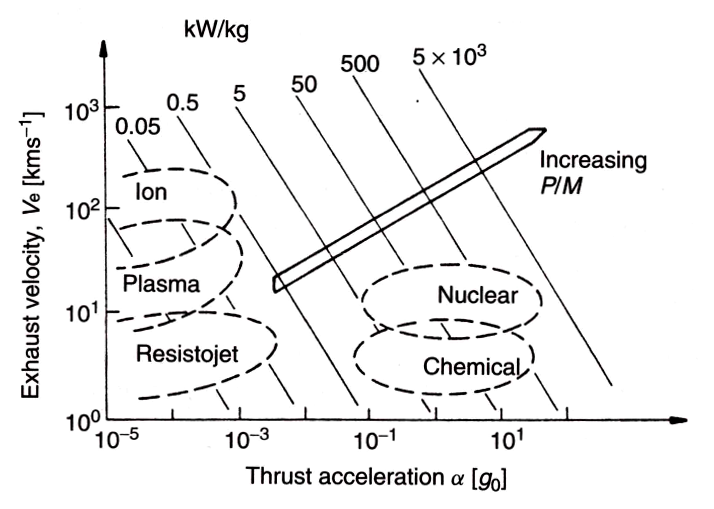
\includegraphics[width=1.0\textwidth]{figures/propulsion-diagram.png}
\caption{Performance characteristics of spacecraft propulsion methods according to energy source.}
\label{fig:propulsionchart}
\end{figure}

\todo[inline]{Concepts: specific impulse, effective exhaust velocity. Influence of the Tsiolkovski equation as said in the Encyclopedia article, mass of the spacecraft. Patel, chapter 23. Sutton 2001, chapter 19.}

Figure \ref{fig:propulsionchart} displays a graphical summary of performance characteristics of several spacecraft propulsion methods according to their energy source.

\todo[inline]{translate, expand, recover references}

Sin embargo, aunque estos sistemas son más eficientes en términos de la masa de propulsante consumida para una trayectoria dada, debido a la limitación de potencia eléctrica disponible a bordo del satélite, las tecnologías existentes producen empujes mucho menores que los disponibles con cohetes químicos y por tanto operan durante períodos de tiempo más dilatados. Este hecho hace que las trayectorias de vehículos propulsados por sistemas de bajo empuje (low thrust) no puedan ser estudiadas como arcos balísticos, y por tanto, requieran un tratamiento analítico mucho más complicado; en particular, existen infinitas trayectorias posibles entre dos puntos (tantas como leyes de guiado se puedan aplicar) [Woodcock, 2002].

\section{The perturbed two-body problem}

\todo[inline]{Derive equations}

\section{Trajectory optimization}

\section{Numerical techniques}

\todo[inline]{Expand}

http://www.maia.ub.es/dsg/wsem/documents/low-thrust.pdf

\textbf{Direct Method}
Solve the Two-point Boundary-value Problem.
Advantage: the solution is smooth and accurate
Disadvantage: Difficult to converge, Difficult to give a reasonable initial guesses 

\textbf{Indirect Method}
Transform the optimal control problem into parameter 
optimization by discretization.
Advantage: Easy to converge than indirect method, some other optimization parameters can be added
Disadvantage: Time consuming, the solution is not smooth 

\textbf{Hybrid Method}
Neglect the transversality condition, adjust the costates by using parameter optimization method (SQP)
It is a tradeoff method between indirect and direct method

\section{Orbital mechanics software}

\todo[inline]{Better explained in Conway}

\begin{itemize}
\item Orekit https://www.orekit.org/static/apidocs/org/orekit/forces/maneuvers/ConstantThrustManeuver.html
\item GMAT 
\end{itemize}

\subsection{Python} \label{sec:python}

\begin{figure}
\begin{lstinputlisting}[language=Python]{examples/algorithm.txt}
\end{lstinputlisting}
\caption{Fragment of BMW-Vallado algorithm for Lambert's problem in Python. Notice its resemblance to pseudocode.}
\label{fig:python}
\end{figure}

The Python programming language was started by Guido van Rossum in 1989 as a successor to the ABC language, and v1.0 was released in 1994\footnote{http://python-history.blogspot.com.es/2009/01/brief-timeline-of-python.html}. It is therefore not new, and in fact it predates the Java language, first released in 1996. On the other hand, Python first uses for scientific purposes appeared as early as 1995, with the creation of a special interest group on numerical arrays\cite{millman2011python}. However, in recent times the ecosystem has greatly improved, with the application of Open Development principles, the increasing interest and involvement of private companies and the generous funds given to projects like IPython\cite{perez2007ipython} and Jupyter. Nowadays, it is one of the most used languages in fields like Astronomy\cite{momcheva2015software} and small-to-medium Data Science, and heavily trusted for teaching undergraduate Computer Science in top universities\cite{guo2014python}. In figure~\ref{fig:python} we can see a fragment of one of the Bate-Mueller-White algorithm to solve Lambert's problem implemented in Python.

One of the most important differences between Python and compiled languages like Fortran or C is its dynamic typing nature. The variety of type systems across has traditionally been a major source of debate among programmers, and in fact some studies suggest that there is "a small but significant relationship between language class and defects"\cite{ray2014quality}. Languages featuring dynamic typing, as it is the case with Python, are often easier to write and read but more difficult to debug, as there are no guarantees about the types of the arguments, and have worse performance. While there is an increasing interest in developing type inference systems (see for instance the Julia and Scala languages), these are extremely difficult to set up for languages like Python \cite{cannon2005localized}.

\subsection{poliastro}

The code developed for this Master thesis is based on \verb|poliastro|, an open source, pure Python library for Astrodynamics and Orbital Mechanics focused on interplanetary applications and released under the MIT license\cite{cano2017poliastro060}. To overcome the limitations mentioned in \ref{sec:python} regarding the performance of the Python programming language, \verb|poliastro| relies on \verb|numba|, an open source library which can infer types for array-oriented and math-heavy Python code and generate optimized machine instructions using the LLVM compiler infrastructure\cite{numba}.

numba works by inferring the types of the variables of a Python function and refining them in several stages until it generates assembly code for the desired platform. In figure~\ref{fig:numba} we see a small fragment of the code that implements the Stumpff functions in poliastro along with its so-called Numba Intermediate Representation, which is the first stage of the optimization process.

\begin{figure}
\begin{lstinputlisting}[language=Python]{examples/annotations.txt}
\end{lstinputlisting}
\caption{Example of numba annotation along corresponding line of Python code.}
\label{fig:numba}
\end{figure}

In \cite{cano2016icatt} detailed benchmarks were conducted to compare the performance of core Astrodynamics algorithms written in Python as featured in \verb|poliastro| and in Fortran. The tests were performed in a virtualized CentOS machine to avoid interferences from the outside world and provide homogeneous results. The results are summarized in table~\ref{table:results}.

\begin{table*}
    \centering
    \begin{tabular}{ c|c c c c c }
          \textbf{Version} & \textbf{Minimum} & \textbf{Maximum} & \textbf{Median} & \textbf{Relative} & \textbf{IQR} \\
    \hline
        \textbf{Intel ifort}, \verb|-O2| & 594620.8 & 654121.4 & 623536.2 & \textbf{1.0} & 25861.2 \\ 
        \textbf{GNU gfortran}, \verb|-O2| & 358478.2 & 505127.0 & 454613.6 & \textbf{0.729} & 68265.5 \\ 
        \textbf{poliastro}, numba & 197610.9 & 206153.2 & 203615.8 & \textbf{0.327} & 3296.5 \\ 
        \textbf{poliastro}, pure Python & 3502.7 & 3703.0 & 3639.6 & \textbf{0.006} & 65.6 \\ 
    \end{tabular}
    \caption{Benchmarking results}
    \label{table:results}
\end{table*}

On the other hand, \verb|poliastro| relies on well-tested, community-backed libraries for low level astronomical tasks, such as Astropy\cite{robitaille2013astropy} and jplephem. Astropy provides several utilities for handling astronomical times and performing reference frame conversions and also allows the user to introduce quantities directly with its physical units, improving the usability of the API\todo{explain what API is somewhere} and reducing the probability of unit errors. jplephem, on the other hand, presents a Python layer to interact with the JPL ephemeris files to compute the position and velocities of the celestial bodies with high precision.

\section{Contribution of this Master thesis}

\todo[inline]{translate, complete}

Si bien en teoría siempre se pueden utilizar métodos numéricos para simular estas trayectorias, en la práctica disponer de soluciones analíticas resulta conveniente para proporcionar una primera solución a algoritmos iterativos, formular problemas de optimización de forma más sencilla o para validación y verificación. Dichas soluciones analíticas son difíciles de encontrar, pero se han desarrollado para varios casos particulares (véase [Di Carlo, 2016] para un resumen de ellos).

Por otra parte, aunque existen algunos desarrollos que implementan uno o varios de estos algoritmos (de nuevo [Di Carlo, 2016] presenta un paquete de optimización escrito en MATLAB), no hemos podido encontrar programas disponibles bajo licencias libres. Al margen de las implicaciones éticas del software libre, sería deseable contar con una versión de estas soluciones reutilizable, fácil de obtener y directamente auditable por una audiencia amplia, con el objetivo de remediar posibles fallos y aumentar la calidad del código.

Por último, nuestras leyes de guiado están acompañadas de casos de validación disponibles en la literatura, con el objetivo de dejar constancia, por una parte, del margen de error entre nuestra implementación y los artículos consultados, y por otro servir de guía para que desarrollos futuros mantengan o mejoren dicho margen de error.

\clearpage